\chapter{~}
What a year!

So far this year, I've relocated to the Louisville area, started casting, photographing and
sketching beautiful women. I've been investigated by undercover police, and nearly been blown
away by a tornado. That is enough to call it a busy year, but there is more.

There is Monique.

Monique is amazing. I realize I've only known her for a few months, and I remember too well
that fact that I didn't like her much at first. My first impressions of her had been wrong,
except for the ones about her being beautiful, and looking like she'd be fun to cast. If only
I'd known then just how much fun casting her was going to turn out to be!

She's at work now, and I find myself standing here in the basement, in the room next to
where we'd gone for protection during the storm. Among me are the cutoff casts that she has
worn, or at least most of them. A few, including her fantastic double shoulder spica, are
somewhere in a Northern Ohio landfill. Still, the collection around me is quite nice: long leg
casts, long arm casts, body jacket casts, and even the awesome half body cast that really
started us down this road. I'm in love with Monique. It's ridiculous to feel this way about
someone I haven't known for very long, but I am in love with her, just the same. I'm not sure
where this road is going to lead, but I'm enjoying the journey. I had a sudden idea, and went
upstairs and called my contact at the medical supply house.

\begin{thought}
Monique was busy at work, but every free moment her mind got, she thought about the
upcoming weekend. She worked every other weekend, building up her savings for the upcoming
school year, which was starting in less than two months. But she wasn't putting every spare
moment of thought into her studies tonight. She was thinking about the weekend coming up. She
was off from work, and she and Quinn were going on a short trip. Nothing fancy, just a couple
hours up the road to Indianapolis. Not exactly a vacation Mecca. Still, there were some
interesting sights to see there.

Sights even nicer to see if you were wearing casts.

The hotel was booked, and the plans were in place. This was going to be a three part
adventure. They would check in at the hotel on Friday morning, go to the room, and use her
random technique to determine an ``injury'' to be treated. After she was casted, they would go
out
and do some publicking. Friday night, they would randomly determine a new ``injury'' and head
out
Saturday with the new cast added to what she had. Saturday evening, they would add the third and
final cast, for what should be the best day of publicking on Sunday. When planning the trip,
they'd agreed on a few basic rules, of sorts: Whatever injury the numbers indicated, they'd go
with, whether it was broken fingers or a cervical vertebra fracture. Also, if the same fracture
repeated itself, they would accept it. So, each day should bring an additional cast, but it
wasn't guaranteed. Sunday morning might find her in nothing more than a short arm cast, or it
might find her in some sort of body cast.

She found herself hoping for a body cast. In fact, she was hoping for a double hip spica.
This was supposed to be a ``holy grail'' of casts to wear, and for her it certainly was. She
could
imagine the whole casting process: the smooth stockinette being applied to her legs and torso,
the gentle pressure of the padding being wrapped, the smell of the fiberglass or plaster as
Quinn wrapped and molded it to her body. She imagined the feel of her waist and hips being
firmly encased in an immovable shell. She wondered if Quinn would want to cast her seated, lying
flat or somewhere in between. She wondered if Quinn would bring the cast over her breasts or
not. She loved the feeling of having her chest casted, but she also loved the feeling of having
it exposed to Quinn later, too. Whatever this weekend brings, she knew she wanted a double hip
spica soon. She had her entire upper body casted, she'd had the left side of her body casted, it
was time to have the lower half casted.
\end{thought}

Friday morning arrived, and I woke up shortly after sunrise. Monique was already awake, out
of bed, and busy. She was dressed in Jean shorts, tank top, and sandals, and she was carrying
the bags we'd packed last night down to load into the SUV, which was already loaded down with
more casting supplies than we'd need as well as crutches and a wheelchair. Since we really
didn't know what sort of ``hardware'' she'd end up in, I made sure to bring the reclining
wheelchair, just in case.

``Wow, you're certainly busy, aren't you?'' I asked sleepily.

``Yes, and you need to be, too! The day is wasting.'' She replied.

I smiled, and hauled myself out of the bed; she came over and gave me a quick kiss, and
then pushed me gently in the direction of the shower. When I was finished and dressed, we headed
out, deciding to get breakfast along the way.

The day was beautiful: sunny, with no clouds. The drive through the farms and countryside
of Southern Indiana was smooth and uneventful. We stopped at a restaurant when we were about
halfway to Indianapolis. Our waitress was a matronly lady of about fifty. She was very polite,
and a good waitress. Amusingly enough, she had a black short arm cast on her left arm. When she
brought our food, Monique asked her ``What happened to your arm?''

``Oh, honey, I slipped and fell on my back steps. I'm lucky I didn't break my neck.''

``So, how long do you have to wear the cast?'' Monique asked

She didn't seem fazed by the question, though I thought it sounded almost prying.

``I've had it on for a month, now. I get checked out next week, and hopefully, I'll get rid
of it then. It's such a pain in the neck,'' she answered.

``Yes, I know what you mean.'' Monique answered. ``My casts have always been bigger than that
one, but I can see how it can make your job more difficult.''

I watched for the response. Monique can be a bit brazen at times, and she was definitely
looking for a certain response. Monique had baited her a bit. If the intent was to shock her, it
didn't quite work. At least not yet, anyway.

``Oh? What kind of cast did you have, dear?''

``Let's see,'' Monique started, ``I've had a below the knee cast a couple of times, full leg
casts four times on the left leg, three times on the right, I've broken my left arm three times,
my right arm twice, and I even had a body cast once.'' She said this almost nonchalantly, as
though everyone had been in casts that often.

``Oh my goodness! What happened to you?''

``Oh, most of them were gymnastics injuries, a couple of auto accidents, and I fell from a
horse, once.'' Monique was creating quite the story on the spur of the moment, which anyone who
is going to public in casts should be prepared to do. Anyone might ask questions at any time
Monique said it with such confidence that I wouldn't have doubted her if she'd been saying it to
me.

``Goodness, girl, you must be accident prone. You be more careful from now on!'' she said as
she left to attend to a couple that had just sat down.

``You know you're horrible.'' I said with a smile after the waitress had left.

``No, I'm just getting into character for the weekend,'' Monique answered. ``Besides, I think
I may have just made her feel better about her situation. And I'm starting to get an idea.''

``Oh boy, here it comes,'' I replied with a smile.

She threw her napkin at me playfully. ``Just what is THAT supposed to mean?''

``Your 'ideas' can be dangerous.''

``What? Sweet, innocent me? Dangerous?'' She said, batting her eyes. ``No, I was just
thinking- if she can wait tables wearing a short arm cast that she hates, I should be able to do
it wearing one that I like.''

``Term cast?'' I asked between bites.

``Sure. Why not?''

``Muscle atrophy for one thing. There are also other bad things that can come from being
casted long term. I'd rather we just keep things short term.''

``I'll talk you into it.'' She said. She just might, too.

We finished our breakfast, and got back on the road. I made sure that we left our waitress
an especially good tip, since we'd had a bit of fun at her expense.

We arrived at the hotel by 9:00 am. The hotel was the perfect home base for our adventure:
It had several entrances, so we could come and go without passing the front desk. It also was a
moderately priced hotel, so there were no bellboys to carry our luggage. These two features
eliminate or decrease any contact that the hotel staff will have with Monique, so we shouldn't
get any uncomfortable questions about the daily changes in her ``medical condition.'' I had
requested a room with accessibility for the handicapped, so I was able to check in for the both
of us. Our room was on the fourth floor on the back side of the hotel, with a view of the
airport, coded our key cards to allow us to use the elevator, and even gave us a parking tag to
allow us to use the designated parking for the handicapped.

I drove us around to the entrance by our room, and we began unloading our luggage. I packed
the casting supplies in two large suitcases instead of the boxes they came in so that we could
leave them in the room by day without advertising to the housekeeping staff what they were. I'd
even found a small plastic basin that fit nicely in the suitcase that would work as a casting
bucket.

Once we had everything in the room, Monique unpacked the laptop, plugged it in and brought
up her random number generator, and the list she'd made.

``Doctor, are you ready?'' she asked.

``Fire away,'' I replied.

Monique tapped the enter key, consulted the list, and announced:

``Doctor, your patient has fractured her left tibia and fibula.''

``I see. Let's get her to the cast room and get that leg casted right away,'' I answered.
Monique headed for the bathroom while I gathered the supplies we'd need.

The bathroom was a pretty good place to do the casting. It wasn't as good as the room at
home I had set up, and the room at home was going to be much better in a week or two, when my
order from the medical supplier came. Still, this bathroom worked well- it was a bit oversized
to accommodate visitors with disabilities, so it gave us some decent room for casting.

``So,'' I started, unfolding and laying out the drop cloth, ``would the patient prefer to
hobble, wobble or roll?''

``What?''

``Hobble, wobble or roll? Would you like to walk on the cast, use crutches, or ride in a
wheelchair?''

``Oh,'' she chuckled. ``You're the doctor, I think you should decide. I just determine the
injury, you decide the particulars of the treatment.''

I filled the plastic basin with warm water and said ``Alright then, go ahead and lean
against the sink, and we'll get started.

I pushed her shorts up as far as they would go, which wasn't far, as they were short
already. I unrolled a section of the four inch stockinette and slid it all the way up her leg. I
then used the six inch padding and started high on her thigh, wrapping downward, adding extra
layers at the knee. I finished the calf and foot area with four inch padding, making sure to pad
the ankle well.

I put on gloves, and unwrapped a package of four inch plaster splints, as well as four
rolls of four inch plaster bandage. I had Monique hold her foot several inches off of the floor
as I placed one roll of plaster into the water. Before it could quit bubbling, I quickly dipped
several layers of the plaster splint into the water, and then held one end against the back of
her calf with my left hand. With my right hand, I retrieved the roll from the water, and started
wrapping it to hold the splinting in place from mid calf to the ball of her foot. I then took a
walking heel, and used the last of the first roll to hold it in place. The next two rolls were
around the foot and lower leg, making sure to get the ankle strong, and the heel firmly
anchored. I used the last four inch roll was used to anchor the padding and stockinette at the
toes, and worked toward her knee. I held her foot while the plaster set a bit.

``Getting warm?'' I asked.

``Yes, it's pretty toasty around my foot and ankle.''

``OK, I'm going to set this foot down on the floor while I finish the cast, but don't put
any weight on it.''

She smiled. ``Yes, doctor, I understand.

I finished her cast with six inch plaster. I used one roll to cover the knee, and two more
to bring the cast high up on her thigh. I folded over the padding and stockinette at the top,
and one final roll set it in place, and continued down her leg, finishing up near the ankle. I
then dipped my gloved hands in the water and smoothed out the cast from top to bottom.

\begin{thought}
As Quinn smoothed out the drying plaster, Monique was enjoying the treat her senses were
receiving: The smell of the plaster, the sight of Quinn working diligently to smooth out the
long cast. Yes, it was definitely long! And the feel of it was wonderful. The smoothness of the
stockinette against her skin, and the heat of the drying plaster were things she'd been dreaming
of feeling all week. Within a few hours, they'd be out in public, which was something she'd been
looking forward to very much. Wearing casts held a lot of attraction to her: she loved the
feelings of the application, and the special attention she got from Quinn the most. She also
loved trying to get around while wearing casts- trying to overcome whatever obstacles the casts
created. She hadn't been kidding when she'd told Quinn that she thought trying to do her job
while wearing a short arm cast would be a lot of fun. She'd probably make better tips, too.

Going out in public while wearing casts was a totally different thrill for her. To her, she
enjoyed the whole charade of acting like she'd actually been injured. She loved when people
would stare, or sneak extra looks at her when they thought she wasn't looking. When someone
actually questioned her, it was the best: she had to tell them a story that they would believe.
She hated lying and deception, but to her, this was different. This was acting, and she enjoyed
the role of the broken lady, with Quinn along to help her through her ``ordeal.'' This morning
at
the restaurant, when she'd told the waitress about her casts she'd had, she knew what she was
saying was way out of the ordinary, yet people who are not ``casters'' aren't likely to question
a
cast, or a story about injury, even if it is very outlandish, and she'd thought her story this
morning had certainly been outlandish. Yet, when she'd seen the look in the eyes of the
waitress, she was thrilled at how convinced shed been. She was hoping this weekend would bring
more of this, and she was certain that it would. As Quinn now wiped the plaster drippings from
her toes and upper thigh, she smiled. Yes, this weekend was going to be great!
\end{thought}

When we'd come in, I hadn't brought crutches or the wheelchair because I didn't know what
sort of cast Monique was going to get today. I slid the drop cloth out from under the heel of
her cast, and folded it up neatly with all of the plaster wrappers inside. I then put it into a
trash bag I'd brought along, and excused myself to the truck to dispose of the bag and retrieve
her crutches. When I returned and gave her the crutches, she moved out of the bathroom and
checked the time.

``Wow, it's not even lunchtime, yet.'' She said.

``We've got plenty of time, thanks to you waking us up so early,'' I joked.

``Hey, I've been looking forward to this all week. I was a bit anxious. Give me a break,
OK?''

``Actually, you gave yourself the break,'' I said, pointing to her casted leg. ``I just
treated it.''

``Yes, and the treatment is very nice. I like this quite a bit,'' she said, looking down at
her leg. ``How long until we can go out?''

``We ought to give it another couple of hours. Let's wait until about noon, go grab
something to eat, then we can hit the art museum.''

We spent the next hour and a half sitting and talking. The cast was damp to the touch by
this time, but the surface was still fragile. I laid down another drop cloth so she could rest
her leg without any of the plaster rubbing off onto the bed.

For lunch, we drove downtown and found a restaurant that had outdoor seating near the
sidewalk. Lunch hour on a warm Friday provided her with quite an audience while we ate. Many,
many passersby did double takes, and others snuck extra looks at her, while a few just plain
stared. We found it quite amusing. From there, we drove to the art museum, which I'd heard good
things about, but had never visited before. The galleries were on three levels, and we'd been
invited by employees to use the elevator, but Monique smiled and just crutched her way onto the
escalator when we wanted to change levels.

The art museum was everything that I'd been told: there were works from most all of the
``old masters,'' and some phenomenal work from some lesser known artists. They had special
galleries devoted to Asian, African, and contemporary art. Of course, there was the
pretentiousness in some of the descriptions that had always amused me about the art world: I
often found it hilarious that someone could seriously tell me that a piece of modern art
represented ``the struggle of man against his environment,'' when it looked to me like someone
had
simply vomited on a canvas and called it finished. Still, some of the works truly inspired me,
and an idea began to form in my head.

Art museums and libraries are places where I can completely lose track of time if I allow
myself to, and today was no exception. Monique and I spent the entire afternoon moving through
the halls, chatting about the work that we liked, and joking about the ones we didn't. When we
went to leave, we were surprised at the late afternoon sun, and we checked the time, and
couldn't believe we'd spent so much time there.

As we made our way back through the parking lot, I noticed a stone wall between the lot and
the grass and trees beyond. I asked Monique to go sit on the wall while I got my pencil and
sketch pad. When I returned, she was sitting with her ``good'' foot on the wall and her casted
leg
stretched out in front of her. I sat across from her, and did a quick sketch. She looked
fantastic in her tank top, shorts, and of course, the cast. My idea from earlier was still
playing in my head as I did this sketch. This really wasn't going to be the finished work, but
the rest of it would come later.

\begin{thought}
Monique watched Quinn attack the paper with his pencil. She felt as though this was
something she could never get tired of watching. Touring the art museum had really made her
think of her father a lot. She'd been so wrapped up in the art, their conversations and her
thoughts that she really hadn't paid much attention to the reactions she got from the other
visitors. She noticed a gawker or two, but mostly it was just a great day out with Quinn.
\end{thought}

As I worked, a few people walking by stopped to look at what I was doing. A few of them
wanted to chat a bit. It was a bit distracting, but I didn't mind too much. Thinking about the
idea I had earlier, I asked one of them where the best place locally to buy art supplies would
be. He directed me to a little shop across town a bit. I got some quick directions, and thanked
him.

When we were back in the truck, I told Monique I had an idea, and wanted to stop at an art
supply store before we went to dinner.

``Did someone get inspired today?''

``Yes,'' I responded, ``I did.''

``All of that art really got you thinking, didn't it?''

``Yes. That and a woman whose beauty begs to be immortalized in art.'' I smiled. Monique
laughed.

The art supply store was in a small trendy area called Broad Ripple. The whole ``village''
appeared to almost be a city within a city. All of the shops were small, and the houses were
older and very well kept. There were many people walking along the streets. It looked like it
might be a promising place for publicking.

We found the art store, and I went in alone. I didn't want Monique to see what I was
getting- I wanted the end result to be a surprise.

I returned with what I'd been looking for, put the bag in the back seat and we headed off
to find a promising looking restaurant.

``So, what did you get?'' Monique asked.

``Let's just let it be a surprise.''

We found a promising looking restaurant for dinner and were not disappointed. The food was
good, and there were plenty of people there for Friday dinner. Monique would have gotten a lot
of second looks without the cast, but it certainly magnified things considerably. There was one
guy who either had a cast fetish or a bladder issue, as he must have walked past us going from
his table to the restroom at least 5-6 times, looking over at her every time he passed.

After dinner, we headed back to the hotel, and decided to relax for a bit before making our
``preparations'' for the next day.

I took my bag from the art supply store, and my sketches from earlier. I took a set of
pastels and a package of colored pencils from the bag, and began recreating the scene from
earlier, but this time in color.

``Oh, nice! Color!'' Monique said.

``Yes, I decided I wanted to try it out.''

After a short bit, Monique got up and hobbled over to her laptop.

``Let's see what my next injury is.'' she said.

\newpage
\begin{center}
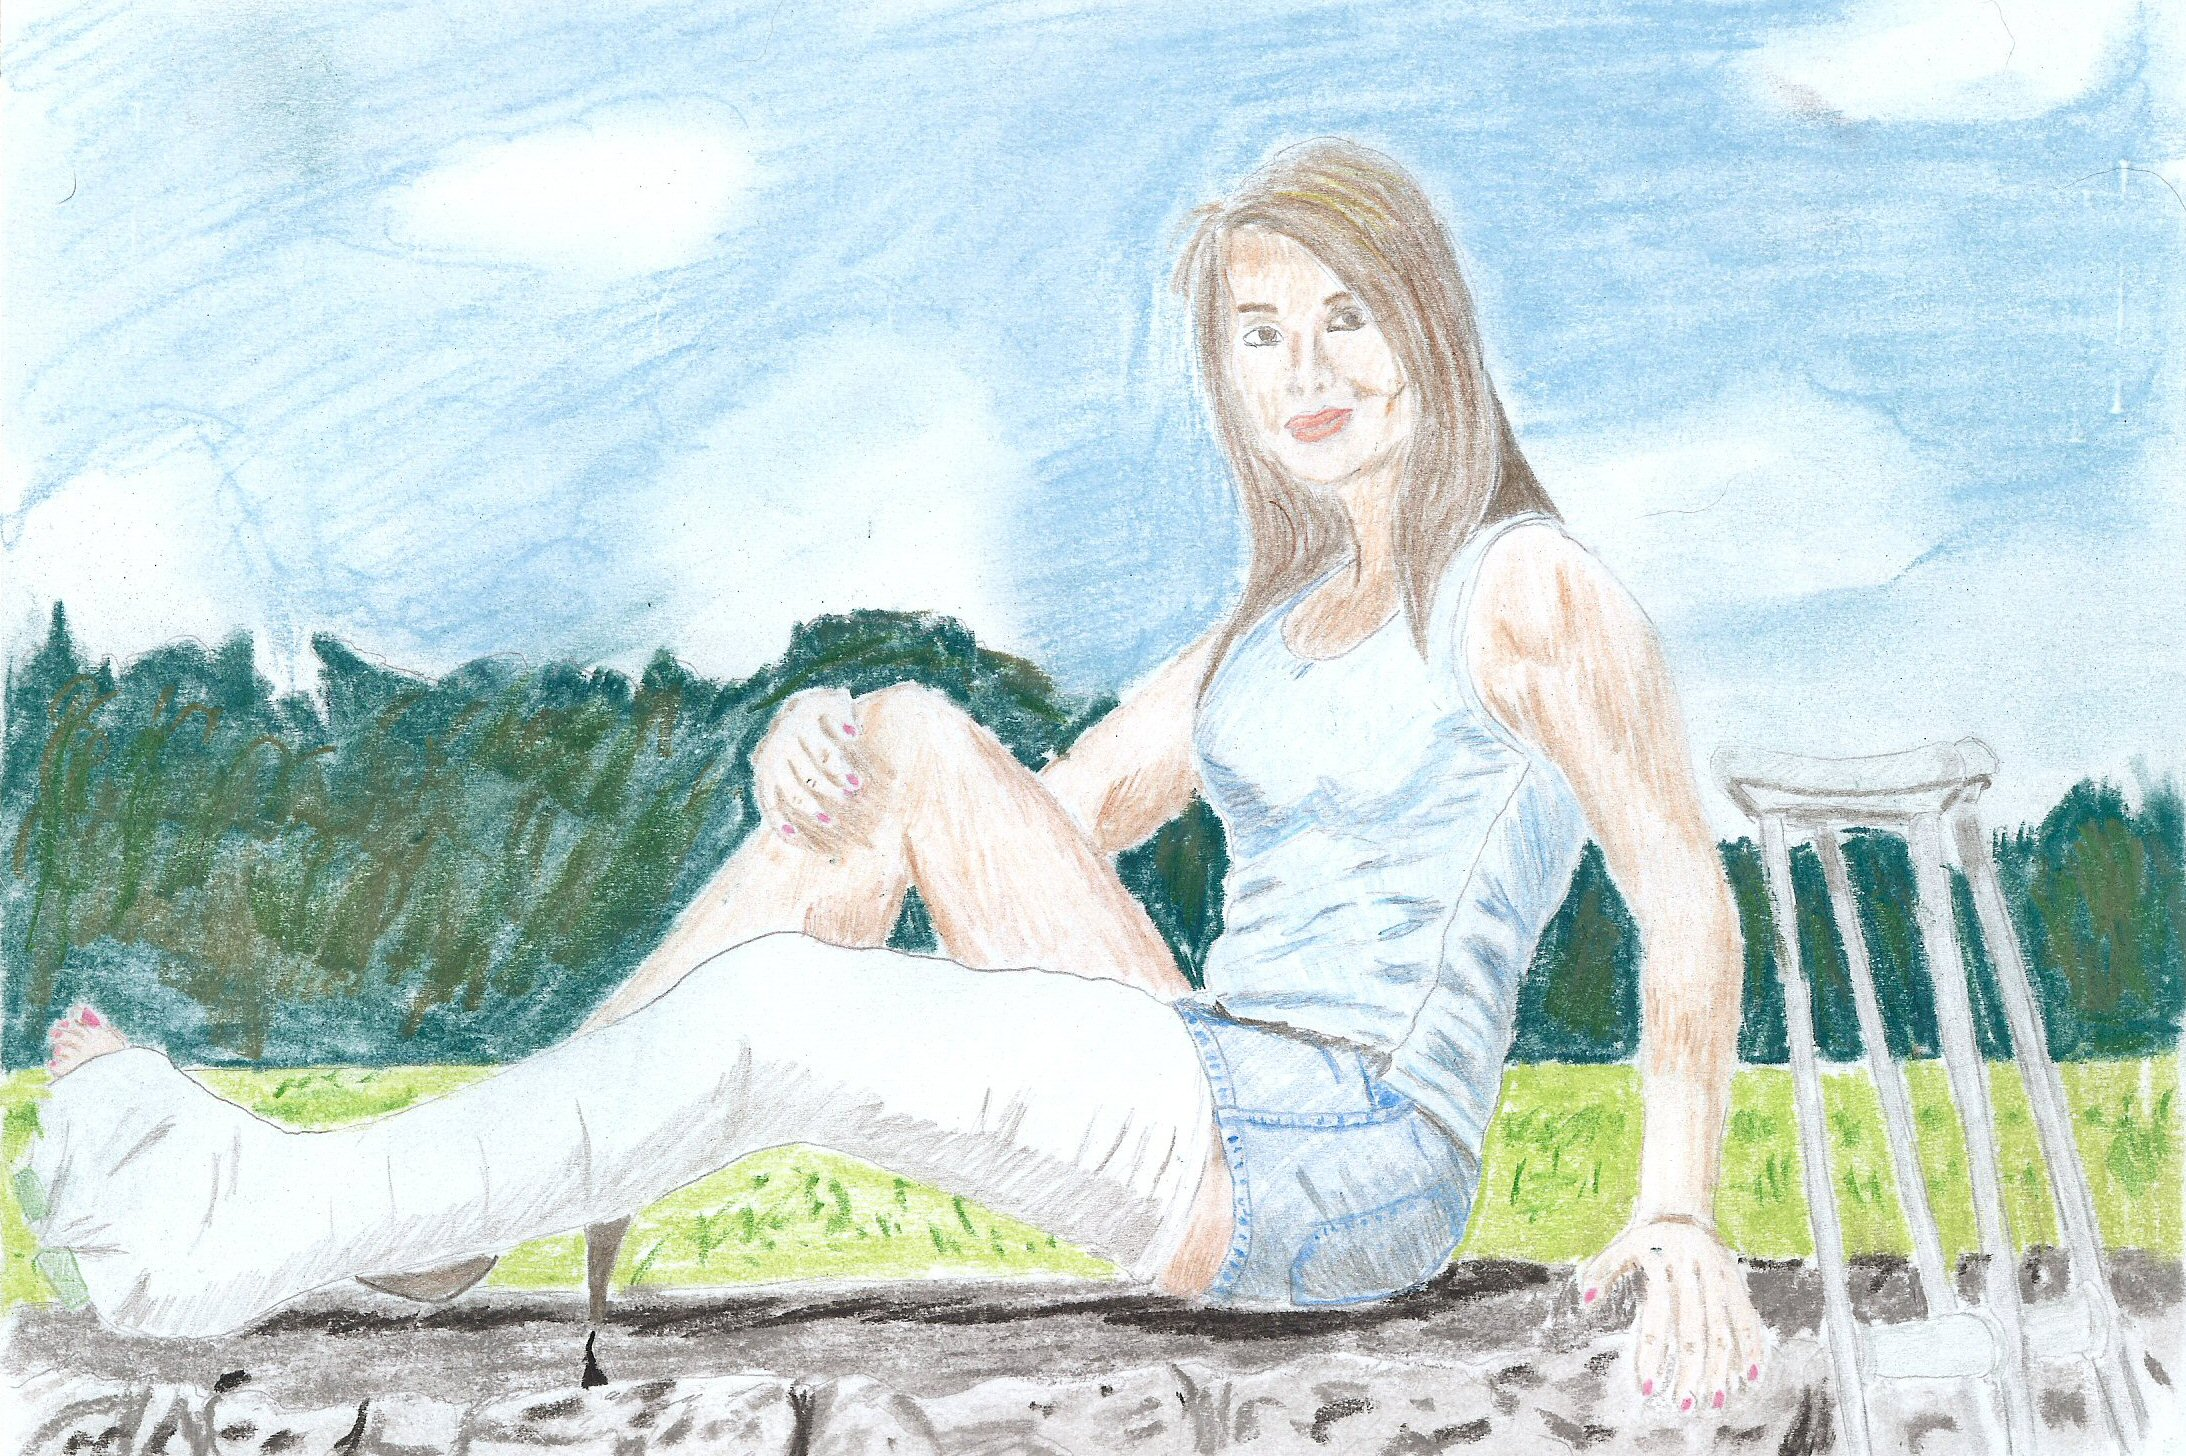
\includegraphics[width=\textwidth]{images/kicks37.jpg}
\end{center}
